\documentclass{article}
\usepackage[utf8]{inputenc}
\usepackage{amsmath}
\usepackage{multicol}
\usepackage{amsfonts}
\usepackage{graphicx}
\usepackage[left=0.25in,right=0.25in,top=0.25in,bottom=0.5in]{geometry}
\newcommand{\ind}{\perp\!\!\!\!\!\!\perp}

\begin{document}

\section{Performance Equations and Power}
\subsection{Performance}
\begin{multicols}{2}
    \begin{itemize}
        \item $\text{Performance} = \frac{1}{\text{Execution Time}}$
        \item $\text{Speedup, B over A} = \frac{\text{Performance}_B}{\text{Performance}_A}$
        \item $\text{Performance Improvement} = \text{Speedup} - 1$
    \end{itemize}
\columnbreak
    \begin{itemize}
        \item $\text{Execution Time} = \text{Cycle Time} \times \text{Cycles}$
        \item $\text{Cycles} = \text{Instructions} \times \text{CPI}$
        \item $\text{Clock Speed} = \frac{1}{\text{Cycle Time}}$
    \end{itemize}
\end{multicols}
\subsection{Power}
\begin{itemize}
    \item $\text{Total Power} = \text{Dynamic Power} + \text{Leakage Power}$
    \item $\text{Dynamic Power } \alpha \text{ Activity} \times \text{Capacitance} \times \text{Voltage}^2 \times \text{Frequency}$
\end{itemize}
\textbf{Allocate array of five 32-bit integers}
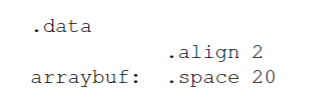
\includegraphics[width=0.30\linewidth]{allocate_array.png}
\section{Memory}
\subsection{Memory Organization}
\begin{enumerate}
    \item \textbf{Scratchpad}: holds a number of values for extremely fast access by the processor, made up of 32 \textbf{registers}
    \item \textbf{Register}: element of a scratchpad, holds 32 bits - can either be a primitive value or an address in memory
\end{enumerate}
\subsection{Procedures}
\begin{enumerate}
    \item \textbf{Activation Record}: area on the stack allocated by a procedure, \$fp points to the start of the activation record and \$sp points to the end.
    \item \textbf{Arguments}: \$a0 to \$a4 are populated with arguments Procedure A wants to call Procedure B with.
    \item \textbf{Return}: when Procedure B returns, it needs to put the return value into \$v0 or \$v1 and hand control back to Procedure A
    \item \textbf{Jump and Link}: \verb|jal Bstart| jumps and hands control to procedure \verb|BStart|
    \item \textbf{Jump Register}: \verb|jr $ra| jumps to the register \verb|$ra|, which holds the return address.
    \item \textbf{Scratchpad}:
    \begin{enumerate}
        \item Caller should save \$ra, \$a0..., \$t0... \$fp (if required).
        \item Callee should save \$s0...
    \end{enumerate}
\end{enumerate}
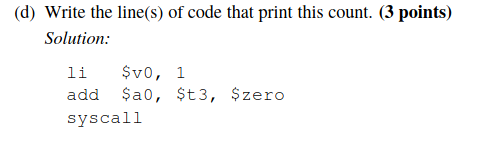
\includegraphics[width=0.50\linewidth]{print_value.png}
\section{Numeric Representations}
\subsection{Unsigned Integers}
\begin{enumerate}
    \item \textbf{Decimal Numbers}: $3512 = 3 \times 10^3 + 5 \times 10^2 + 1 \times 10^1 + 2 \times 10^0$
    \item \textbf{Binary Numbers}: $10101 = 1 \times 2^4 + 0 \times 2^3 + 1 \times 2^2 + 0 \times 2^1 + 1 \times 2^0$
    \item \textbf{Hexadecimal}: $\text{0x19af} = 1 \times 16^3 + 9 \times 16^2 + 10 \times 16^1 + 15 \times 16^0$
\end{enumerate}
\subsection{Signed Integers}
\begin{enumerate}
    \item \textbf{Binary Numbers - Two's Complement}: first bit represents sign; the rest counts up from 0 (when positive) and up from $-2^{31}$ (when negative)
    \begin{multicols}{2}
        \begin{itemize}
            \item $0000...0000 = 0$
            \item $0111...1111 = 2^{31} - 1$
            \item $1000...0000 = -2^{31}$
            \item $1111...1111 = -1$
        \end{itemize}
    \columnbreak
        \begin{itemize}
            \item $x_{31} x_{30}...x_{0} = -2^{31}x_{31} + 2^{30}x_{30} + 2^{29}x_{29} + ... + 2^0x_0$
            \item Addition can be done just like decimal
            \item Let $\overline{x}$ be $x$ with bits inverted.
            \item $-x = \overline{x} + 1$
        \end{itemize}
    \end{multicols}
\end{enumerate}
\subsection{Floating Point Numbers}
\begin{enumerate}
    \item \textbf{Single-Precision Floating Point}:
    \begin{enumerate}
        \item Put the number into scientific notation in binary, of the form $\pm 1.\text{fraction} \times 2^{\text{exponent}}$. Bits go from 31 to 0, left to right.
        \item Bit 31 (S) stores the sign, 0 for positive and 1 for negative
        \item Bits 30-23 (E) stores (exponent + bias) as an unsigned int, bias is $127$
        \item Bits 22-0 (F) stores the fraction section (right of the point) of the number, trailing 0s are added to the right as needed.
        \item \textbf{Addition}: normalize the smaller exponent to match the larger exponent, add the fractions
    \end{enumerate}
    \item \textbf{Double-Precision Floating Point}: same as single-precision, but 11 exponent bits, 52 fraction bits, bias is 1023.
\end{enumerate}

\section{Digital Design}
\subsection{Boolean Algebra}
\begin{multicols}{3}
    \begin{itemize}
        \item \textbf{OR}: A + B $\iff$ A or B
        \item \textbf{AND}: A.B $\iff$ A and B
        \item \textbf{NOT}: $\overline{A} \iff$ not A
    \end{itemize}
\columnbreak
    \begin{itemize}
        \item $\overline{A + B} = \overline{A}.\overline{B}$
        \item $\overline{A.B} = \overline{A} + \overline{B}$
        \item $A.(B + C) = (A.B) + (A.C)$
    \end{itemize}
\columnbreak
    \begin{itemize}
        \item $A + (B.C) = (A + B).(A + C)$
        \item \textbf{Sum of Products}: using a truth table, pick all true conditions and OR them together
    \end{itemize}
\end{multicols}
\subsection{Ripple-Carry Adder}
\begin{enumerate}
    \item A 1-bit adder takes in a carry (carry-in), puts out a carry (carry-out), and adds two digits. 
    \item Ripple-Carry connects the adders together; the carry-out of one adder serves as the carry-in of the next adder. This is similar to how we do addition, one pair of digits at a time and carrying when needed.
\end{enumerate}
\subsection{Carry-Lookahead Adder}
\begin{enumerate}
    \item Instead of waiting for the previous adder to put in a carry, we calculate whether there exists a carry ahead of time.
    \item $c_{i + 1} = a_i.b_i + (a_i.b_i).c_i$: $a_i$ is $i^{th}$ bit of a, $b_i$ is $i^{th}$ bit of b, $c_i$ is whether $i^{th}$ bit has a carry
    \item Can chunk bits into 4 - do those 4 bits generate a carry?
\end{enumerate}


\section{Finite State Machines}
\begin{enumerate}
    \item \textbf{Finite State Machine}: the machine takes \textbf{input} and stores a \textbf{state}, using that information to move to a new state
    \item \textbf{Finite State Table}: enumerate all possible permutations of current state and inputs, record the next state that the machine stores (output)
    \item \textbf{Finite State Diagram}:
    \begin{enumerate}
        \item What are possible output states? Draw a bubble for each.
        \item What are inputs? What values can those inputs take?
        \item For each state, what do I do for each possible input value? Draw an arc out of every bubble for every input value to represent a transition to a different state.
    \end{enumerate}
\end{enumerate}

\end{document}
